\section{Resultados e Discuções}


%pré javascript

Nos primeiros dias da \textit{World Wide Web}, um navegador precisava apresentar apenas alguns tipos de dados aos usuários. Para não ser limitado por esses tipos de dados, os desenvolvedores trabalharam duro para estender os navegadores para que dados em outros formatos pudessem ser renderizados no computador cliente. Uma maneira de resolver o problema era permitir que o navegador, ao reconhecer um arquivo recebido de um tipo específico, iniciar um aplicativo separado na máquina cliente para renderizar o conteúdo. Desde que este aplicativo auxiliar tenha sido instalado no computador cliente, o navegador iniciará o programa e enviará o arquivo recebido para esse programa \cite{zammetti2007brief}.

A primeira solução para tornar a web mais dinâmica foi o \textit{"Common Gateway Interface"} (CGI), que permite a criação de programas que executem quando um usuário faz uma requisição. Porem, CGI não é a solução mais segura para criação de páginas web pois permite que seja executado um programa em seu sistema operacional e usuários maliciosos podem explorar isto com algum exploit\footnote{Uma sequência de comandos que tomam vantagem de um defeito, falha ou vulnerabilidade a fim de causar um comportamento acidental ou imprevisto.} e executar operações indesejadas \cite{Asleson2006}.

Ainda segundo \citeonline{Asleson2006}, em maio de 1995 John Gage e Andreessen anunciam o nascimento da linguagem de programação Java. O navegador Netscape era dominante na época e ofereceria suporte para esta nova linguagem. Dentro de alguns meses, milhares de pessoas já haviam baixado o Java em seus computadores, abrindo novos caminhos para páginas web dinâmicas.

Applets\footnote{Pequeno software que executa uma atividade específica dentro de outro programa maior.} permitem que pequenas aplicações Java possam ser incluídas nas páginas web e executadas através da \textit{Java Virtual Machine} (JVM). Applets são executadas no modelo de segurança de "caixa de areia" (\textit{sandbox}), não podem carregar bibliotecas nativas e são tipicamente impedidas de ler ou gravar no disco \cite{Asleson2006}.

Ainda em maio de 1995, Brendan Eich, um funcionário da Netscape\footnote{Empresa de serviços de computadores nos EUA.} na época, desenvolveu uma linguagem de script em dez dias que se tornou conhecida como Mocha. Este nome original foi dado pelo fundador da Netscape. Pouco depois, o nome foi avaliado e renomeado como Livescript. Mais tarde naquele ano em dezembro, a Netscape recebeu uma licença de marca registrada da Sun\footnote{Fabricante de computadores, semicondutores e software com sede em Santa Clara, Califórnia, no Silicon Valley.}. Desta vez, o nome mudou para Javascript \cite{neer2013history}.

Javascript foi concebido para fins muito diferentes do Java, essencialmente para funcionar como uma linguagem de programação integrada em documentos HTML e não como uma linguagem para escrever applets que ocupam uma área retangular fixa na página \cite{goodman2007javascript}. O Javascript tinha um pequeno vocabulário e um modelo de programação mais facilmente digerível que o Java, com sua abordagem orientada a objetos. Nesse contexto \citeonline{crockford2008javascript} afirma que com Javascript é possível programar sem saber muito sobre a linguagem, ou mesmo saber muito sobre programação.

A primeira versão, o Javascript 1.0, estreou no navegador Netscape 2 em 1995. No momento do lançamento do Javascript 1.0, o Netscape dominava o mercado de navegadores. A Microsoft estava lutando para recuperar seu próprio navegador, Internet Explorer e seguiu rapidamente a liderança da Netscape ao lançar sua própria linguagem VBScript\footnote{Versão interpretada da linguagem Visual Basic para construção dinâmica de página HTML}, juntamente com uma versão do Javascript chamada JScript, com a entrega do Internet Explorer 3 \cite{keith2010dom}.

\begin{figure}[!htb]
	\centering
	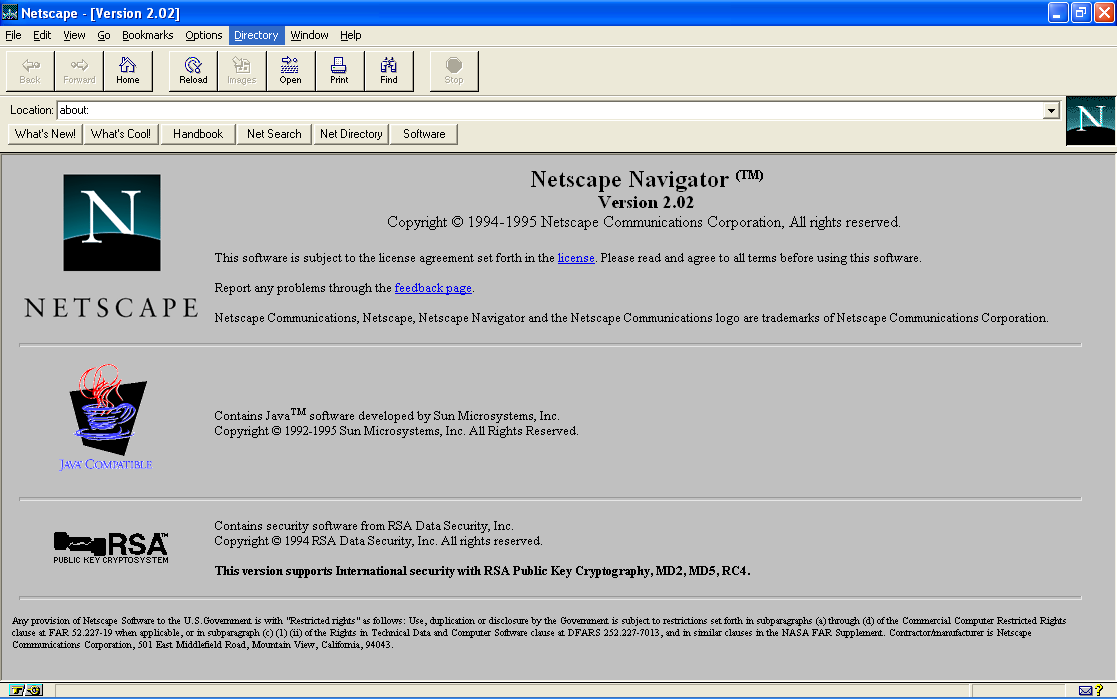
\includegraphics[width=350px]{Netscape_Navigator_2.png}
	\caption{Navegador Netscap 2}
	\label{Netscape}
\end{figure}

A Netscape enviou a linguagem para padronização para a Associação Europeia de Fabricante de Computadores (ECMA) e devido a problemas de marca registrada, a versão padronizada da linguagem estava presa com o nome estranho "ECMAScript". Pelos mesmos motivos de marca registrada, a versão da Microsoft do idioma É formalmente conhecido como "JScript" \cite{flanagan2011javascript}.

O ECMAScript como foi padronizado não se destina a ser computacionalmente auto-suficiente, espera-se que o ambiente computacional de um programa ECMAScript forneça certos objetos específicos do ambiente; um navegador da Web fornece um ambiente de \textit{host} para computação do lado do cliente, incluindo, por exemplo, objetos que representam janelas, menus, pop-ups\footnote{Janela que abre no navegador da internet quando se acessa uma página na web ou algum link de redirecionamento.}, caixas de diálogo, áreas de texto, âncoras, quadros, histórico, cookies\footnote{Grupo de dados trocados entre o navegador e o servidor de páginas, colocado num arquivo de texto criado no computador do utilizador.} e entrada / saída; um servidor web fornece um ambiente de \textit{host} diferente para a computação do lado do servidor, incluindo objetos que representam requisições \cite{ecmascript2016}.

------------------------------------------------------------------------------------
%pré ajax, iframes
\subsection{Pré Ajax}

Em 1995, já era possível construir \textit{Single Page Applications} (SPAs) via frames/framesets\footnote{Divisões internas dentro de uma mesma janela do navegador, onde são carregados outros documentos HTML.} e url="javascript:...". Requisições assíncronas também eram possíveis utilizando Javascript e manipulando elementos HTML que realizavam requisições HTTP; praticamente qualquer tag que possa ser configurado para fazer referência a um URL pode ser empregado para tarefas de comunicação com base em Javascript \cite{powell2008ajax}.

Ainda segundo \citeonline{powell2008ajax}, utilizando-se de tags que referenciam URL é possível gerar uma requisição de via única ao servidor para indicar que algum evento aconteceu através de campos adicionados ao URL (\textit{Query Strings}). Para isso, utiliza-se de parâmetros passados via URL por uma tag\footnote{Estruturas de linguagem de marcação contendo instruções, tendo uma marca de início e outra de fim para que o navegador possa renderizar uma página.} \textit{<img>} por exemplo, cabe ao servidor tratar a requisição e retornar o dado esperado ou uma resposta vazia com status 204, informando ao cliente que a solicitação ocorreu sem erros mas que não há conteúdo na resposta.

Quanto ao uso da tag \textit{<im>} para comunicação bi-direcional \citeonline{powell2008ajax} completa:


\begin{quote}
	Parece que o uso de uma imagem provavelmente não é a melhor maneira de transmitir informações bidirecionais. Considere que, se você pedir uma imagem, você estará recebendo uma imagem, provavelmente em formato GIF, JPEG ou PNG para exibição. Como exemplo, você pode solicitar ao usuário alguns dados e, em seguida, gerar uma imagem personalizada para eles. A transmissão dos dados fornecidos pelo usuário é através da seqüência de consulta como anteriormente, mas desta vez o servidor responderá não com um código 204, mas com uma imagem real para usar. Você pode usar o DOM e inseri-lo na página.
\end{quote}

Visto que um navegador permanecerá na mesma página quando receber uma resposta 204, ele pode ser usado para fingir ir a uma URL apenas para enviar alguns dados; isto é feito em Javascript com uma atribuição direta para \textit{window.location} enviando os dados pela url, através das \textit{Query Strings}. Porem as \textit{Query Strings} são limitadas ao tamanho máximo da URL permitido pelo navegador. Para envio de uma grande quantidade de dados o desenvolvedor precisa realizar uma requisição HTTP POST em uma técnica de iframes\footnote{Elemento HTML que permite carregar as informações de um documento HTML separado em um documento HTML existente.} escondidos. Está técnica consiste da criação de campos de formulário a serem enviados com o formulário inserido no iframe. Uma vez que o formulário é preenchido com os dados desejados, é desencadeado o envio do formulário via Javascript \cite{powell2008ajax}.


\subsection{Ajax}

O termo Ajax é um acronimo para "Javascript assincrono e XML" \cite{Garrett2005} e descreve uma maneira de realizar uma comunicação HTTP a partir de uma aplicação Javascript em páginas web.

% long polling



% http chunk data stream

\subitem{Server-Sent Event (SSE)}

\subitem{Web Sockets}

